\section{Graphical Design}

When you dive into the ocean of possibilities that is design, there are many factors to be considered. What color palette should you choose? And which fonts goes best together. And how do you find your way through mixing the right colors and fonts? And how does this affect the way your design is being perceived? 

\subsubsection{Colors}
There are to primary colours. Additive and subtractive. Additive is used on screens as it gives away light and subtractie is used for e.g. bookcovers as it reflects light. \cite{Colour}
These are also known as RGB(Red, blue and green) and CMYK(Cyan, magenta and yellow).
In additive colours white is colours mixed together where black is the absence of color. In subtractive white is the absence of color and black all the colors mixed together. 
Since subtractive colour do not fully absorb light a fourth element has been added, hence the K in CMYK. K stand for 'key' which essentially is black.\cite{Colour}

The colour wheel can helps us see which colours are complimentary, adjacent and triadic. 
\begin{figure}[H]
\centering
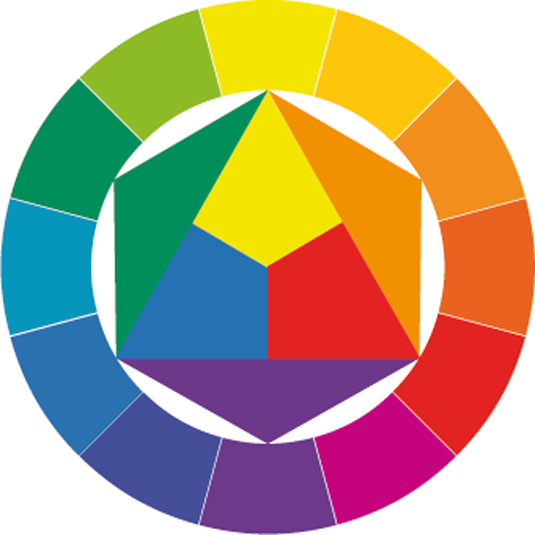
\includegraphics[scale=0.25]{wheel.png}
\caption{The colour wheel. \cite{Colour}}
\end{figure}

Colours are defined by hue, saturation and brightness. 
Using a colour gamut you can see all the different shades available. As you will discover, the RGB is much more limited than CMYK. This is because there is a limit to how much a screen is able to show. 

It is important to remember that when choosing the colour palette for a design that how we perceive colour is very different. Also, colours can change according to what you put it next to. Yellow might look different next to grey than it will next to purple for instances. \cite{Colour}

When it comes to color psychology the truth is it is too dependent on personal experience. There is no one right answer to which color falls into what moodlet. \cite{ColorMeaning}
There is, however, many studies conducted on this matter. 
One study shows that 90\% of people make snap judgement based on colour alone. \cite{ColorMeaning} Another study shows that an intend of purchasing is linked with how a brand is perceived, what kind of "personality" does the brand have?\cite{ColorMeaning}

\begin{figure}[H]
\centering
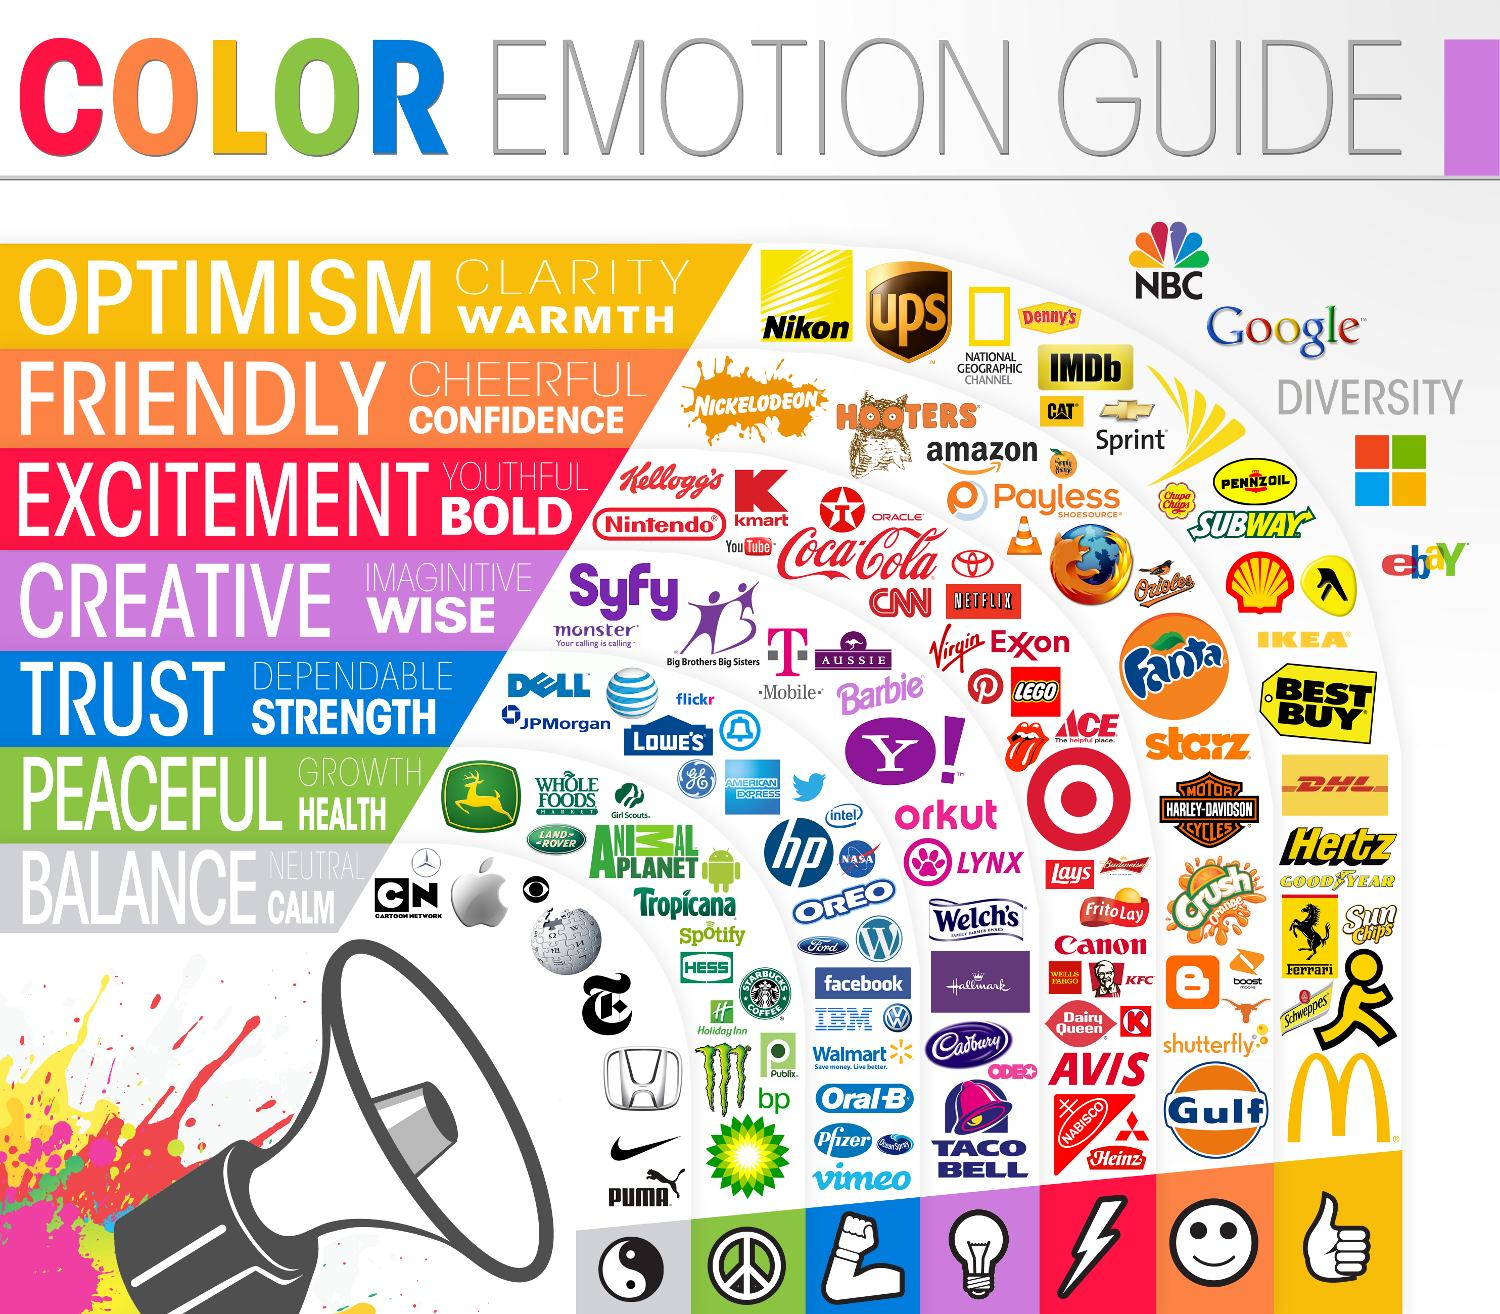
\includegraphics[scale=0.125]{color-emotion.jpg}
\caption{Overall image of how colours are generally percieved. \cite{ColorMeaning}}
\end{figure}

But all in all, the concept you are working with is key. Almost every study shows that it is greatly more important to choose a colour that shows the personality of your product than picking a stereotype colour. \cite{ColorMeaning}

Lastly, colour preferences differ between genders. Women prefer soft colours and tints while men prefer bright colours and shades. \cite{ColorMeaning} 

%something about coordination

\subsubsection{Rythm, Balance and proportions}
Something about rythm, balance and proportions. \cite{DesignPrinciple}

\subsubsection{Fonts}
The most popular combinations of fonts is sans sherif and a sherif body type. \cite{TypeComb}
which font to choose \cite{Font}

\subsection{Design Patterns}
Two of the things people often complaint about in applications is a confusing interface design and poor navigation. \cite{Pattern} This can be prevented by using design patterns. 
First, let's look at navigation. There are two ways to make navigating through an app easier. Persistent and transient. Persistent navigation is your list menus and your tab menus or menu structures if you will. Transient navigation has to be revealed through a tab action or the likes.\cite{Pattern}
Does the user need to see the menu at all times? If not, you can use an off-canvas solution like the side bar. 
It has become more and more popular to use off canvas methods. \cite{Pattern} This helps the app hold more information but without being confusing e.g. If all your information has to go on one page. 
You don't want to put too much text into one page or have a simple form take up several pages. A sign in for example should only be one page. A way to not get an over lapping look is by using vertical labels instead of horizontal. \cite{Pattern} Or you could have the horizontal labels where the text disappears as soon as the user starts typing, but you risk that the user forgets what they should fill in.\cite{Pattern} 
Some apps, like Instagram, shows the "sign in" and "sign up" option all the way through the tutorial. This also insures that the user do not have to go through a whole tutorial if they don’t need it. 
Another important form is the "search" form. This should be very short. It is a good idea to offer a filter option like "saved searches". There are several kinds of searches. 

Explicit search is the most standard search option and is pretty straight forward. But you can still give it a little extra. E.g. When the user chooses the search bar but haven't typed anything in yet you could give them some options in a list e.g. have a "scan" option at the top, latest searches, saved searches etc. \cite{Pattern}

Implicit search will give the user something they didn't search for and what they might not know they needed. E.g. Search for coupons when you enter your local grocery store and give an alert if there is anything useful. This will enhance the user experience as well. \cite{Pattern}

Scoped searches is searching for something more specific. You can choose to search in different categories to minimize the results and not get a result of 1500 different chairs if you are looking for one specific chair. \cite{Pattern}

Lastly there is the dynamic search or dynamic filtering. This is used to minimize choices in set lists like in music library. This is however only good with small data sets.\cite{Pattern}

There are many more patterns and anti-patterns to discover. \cite{Pattern}

Keeping these patterns in mind there are still many things to consider. 
First of all, remember the size of the screen that you are designing for. Avoid using big scaled photos and put to much information at one page. This will make it look cluttered and make it less intuitive. \cite{Graphic}
In short, make everything as clean and simple as possible. 

When designing your layout it is, once again, key to keep everything simple and streamlined. 
Follow the general rules, left-to-right and top-to-bottom. Make sure the most important feature is in the top left corner where the user will look first.\cite{Graphic}

Be careful when choosing a font type. You cant control the devices fonts and thus try to pick an common type font.  \cite{Graphic} To make the text easy to read make sure that the contrast between text and background is present. Either black and white or a light coloured background with dark text. \cite{Graphic}

Last but not least; colors. Make sure that the colors are bright enough and that the contrast is sufficient since the weather can affect the UX. \cite{Graphic}


